\chapter{Representation changes with learning}

To measure how the time representation changes with learning, we will compare the neural activity extracted from distinct learning stages. Specifically, we divide into the first and second half of the session for the group with long sessions, and into the first and second sessions for the group with short sessions. This is because for the first group we had long sessions of more than 1000 trials $(1149 \pm 384)$ with sufficient correct trials $(660 \pm 260)$. For the second group of animals, in which sessions were half as long with $570 \pm 181$ trials, there were only and $284\pm 100$ correct trials, less than half compared to the first group.

We will measure the quality of time representation using the same machine learning techniques from the previous chapter.

\section{Striatum enhances its representation while mPFC decreases}

\begin{figure}[ht]
    \centering
    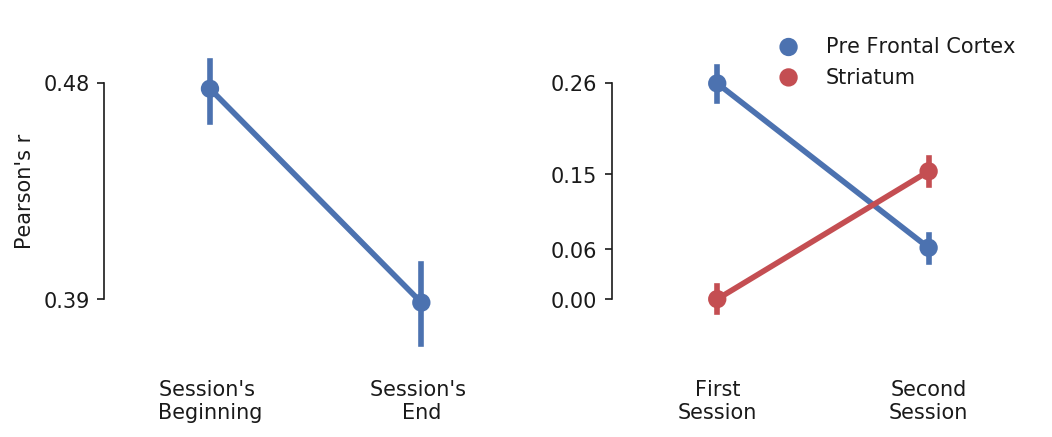
\includegraphics[width=\textwidth]{figures/pearson_comparison_before_after_learning.png}
    \caption[Comparison of classifier performances in distinct learning stages, by Pearson Correlation]{Comparison of classifier performances in distinct learning stages, by Pearson Correlation. Left: Group 1 at first half vs second half of session. Right: Group 2, in the first vs the second smaller sessions. In the vertical, we show the performance of the classifier as measured by Pearson's r. Values shown in the vertical axes correspond to the mean values of data points, shown as circles. The analysis was repeated 100 times, and error bars correspond to the confidence intervals of 95\% calculated by 1000 bootstrap averages of 100 samples with replacement.}
    \label{fig:time_representation_str_pfc}
\end{figure}